% IEEE/ACM Transactions on Computational Biology and Bioinformatics (TCBB)
% IEEE Computer Society journal format (IEEEtran, compsoc).
% Converted from sn-article.tex (Springer Nature sn-jnl).
% Supplementary material (Sec./Fig./Table/Alg. S*) is in ieee-supplement.tex,
% uploaded as a separate file as TCBB requires.

\documentclass[10pt,journal,compsoc]{IEEEtran}

\ifCLASSOPTIONcompsoc
  \usepackage[nocompress]{cite}
\else
  \usepackage{cite}
\fi

\usepackage{graphicx}
\usepackage{array}
\usepackage{booktabs}
\usepackage{multirow}
\usepackage{amsmath,amssymb,amsfonts}
\usepackage{textcomp}
\usepackage{xcolor}
\usepackage{hyperref}

\newtheorem{proposition}{Proposition}

\begin{document}

\title{Benchmarking Single-Cell Marker-State Forecasting Under Independent and Coupled Cell Pairings}

\author{Victor~Ikenna~Kanu (MIEEE),
        Ihunanya~Udodiri~Ajakwe,
        Josiah~Ayoola~Isong,
        Simeon~Okechukwu~Ajakwe (SMIEEE),
        and~Dong-Seong~Kim (SMIEEE)%
\IEEEcompsocitemizethanks{%
\IEEEcompsocthanksitem V.~I.~Kanu, I.~U.~Ajakwe, J.~A.~Isong, and D.-S.~Kim are with the Department of IT Convergence Engineering, Kumoh National Institute of Technology, Gumi 39177, South Korea.\protect\\
E-mail: kanuxavier@gmail.com, ihunanya.ajakwe@gmail.com, isongjosiah@gmail.com, dskim@kumoh.ac.kr
\IEEEcompsocthanksitem S.~O.~Ajakwe is with the Smart Computing Department, Kyungdong University, Global Campus, South Korea.\protect\\
E-mail: simeonajlove@gmail.com
\IEEEcompsocthanksitem All authors contributed equally to this work.
\IEEEcompsocthanksitem Corresponding author: Dong-Seong Kim.}% <-this % stops an unwanted space
% ORCID iDs: V. I. Kanu 0009-0005-5606-8105; I. U. Ajakwe 0009-0004-9922-2320;
% J. A. Isong 0000-0002-6151-1950; S. O. Ajakwe 0000-0002-6973-530X; D.-S. Kim 0000-0002-2977-5964
}

\markboth{IEEE/ACM Transactions on Computational Biology and Bioinformatics}%
{Kanu \MakeLowercase{\textit{et al.}}: Forecasting Under Independent and Coupled Pairings}

\IEEEtitleabstractindextext{%
\begin{abstract}
Models that forecast later differentiation states from earlier single-cell RNA-sequencing snapshots are trained and evaluated on pseudo-trajectories that link cells across time points. Because measurement is destructive, how cells are linked---independently, or through an inferred coupling such as optimal transport (OT)---determines how much temporal information a benchmark contains, yet this is rarely checked, and model comparisons are often single-seed and vulnerable to train--test leakage. A leakage-safe protocol (one shared split, training-only normalization, 20 seeds, paired statistics with an equivalence test, and an input-independent baseline) was applied to iPSC-to-dopaminergic-neuron and iPSC-to-cardiomyocyte time courses. Under independent pairing the late stage is provably independent of the earlier stages, and the protocol recovered this null: a Transformer, a random forest, and ridge regression were statistically equivalent, and all were outperformed by the constant training median ($6$--$7\%$ lower error, neural; $28$--$31\%$, cardiac). A $19.4\%$ Transformer advantage obtained with the pipeline of an earlier study arose from train--test leakage. In positive controls, the same protocol detected recoverable dependence in simulated differentiation with known ground truth, and on both real lineages OT coupling allowed every model to beat the input-free baseline, showing that the protocol detects dependence induced by the chosen coupling, though not that this dependence is biological. The Transformer never significantly outperformed the random forest, and a stage-order shuffle control was insensitive even when dependence was known to exist. What a forecasting benchmark can detect is set by how cells are coupled, not by model capacity; benchmarks should state their coupling, report a metric-matched input-independent baseline, and validate their controls where dependence is known.
\end{abstract}

\begin{IEEEkeywords}
Single-cell RNA-seq, differentiation forecasting, optimal transport, data leakage, equivalence testing, benchmark evaluation.
\end{IEEEkeywords}}

\maketitle

\IEEEdisplaynontitleabstractindextext

\IEEEpeerreviewmaketitle


\IEEEraisesectionheading{\section{Introduction}\label{sec:intro}}

\IEEEPARstart{S}{ingle-cell} RNA sequencing (scRNA-seq) has enabled population-scale characterization of stem-cell differentiation, resolving stage-dependent gene-expression programs across experimental timepoints~\cite{jerber2021population}. A natural ambition is to move from describing these programs to \emph{forecasting} them: given cell states observed at early differentiation stages, predict the state at a later stage. Generative models of single-cell time series aim to predict future cell states and fates from snapshot data~\cite{yeo2021prescient,tong2020trajectorynet}, neural ordinary differential equations (ODEs) have been proposed for continuous-time transcriptomic forecasting~\cite{erbe2023transcriptomic}, and related models learn cellular dynamics with variational--neural-ODE hybrids~\cite{farrell2023inferring} or physics-informed stochastic differential equations~\cite{jiang2024physics}. Transformer architectures developed for annotation and foundation modelling~\cite{chen2023transformer,cui2024scgpt} are increasingly applied to single-cell prediction tasks. Yet when such models have been compared with simple baselines under careful evaluation, particularly in the closely related problem of predicting perturbation responses, they have often failed to outperform linear or even trivial predictors~\cite{ahlmanneltze2025deep,kernfeld2023systematic}. Whether added capacity, especially the capacity to model temporal dependency, improves forecasts of differentiation state therefore requires testing rather than assumption.

Two fronts determine whether a reported improvement is real. The first is the structure of the data. Because single-cell measurement is destructive, no cell is observed at more than one timepoint~\cite{la2018rna}. Metabolic RNA labelling~\cite{erhard2019scslam,cao2020scifate} and lineage barcoding~\cite{weinreb2020lineage} can partly recover temporal links, but standard cross-sectional time courses, including those analysed here, provide neither. Temporal ordering must then be imposed computationally: by pseudotime~\cite{saelens2019comparison,haghverdi2016diffusion}, RNA velocity~\cite{la2018rna,bergen2020generalizing}, optimal-transport couplings between consecutive time points~\cite{schiebinger2019optimal,lavenant2024toward}, or \emph{pseudo-trajectories} that concatenate independently sampled cells in stage order. A pseudo-trajectory is not a tracked lineage; its states are independent draws, so it is unclear whether it contains any temporal dependency for a sequence model to exploit.

The second front is evaluation rigor. Data leakage, the inadvertent sharing of information between training and test partitions, is a pervasive failure mode in machine learning applied to biology that inflates performance estimates~\cite{whalen2022navigating,bernett2024guiding}; a cross-disciplinary survey attributed irreproducible findings to leakage in at least $294$ papers across $17$ fields, often where complex models appeared to beat simple baselines~\cite{kapoor2023leakage}. Model comparisons are also often reported from a single random seed, although both pseudo-trajectory construction and neural-model training are stochastic, and a single-seed estimate cannot distinguish an effect from sampling variation~\cite{pineau2021improving}. Finally, establishing that two models perform comparably requires an explicit equivalence test, because a nonsignificant difference is not evidence of equivalence~\cite{lakens2017equivalence}.

The two fronts interact. How cells are linked across time points determines how much temporal information a benchmark contains at all (Table~\ref{tab:rigor}), and an evaluation that cannot distinguish a model's skill from an artifact of its construction cannot establish whether temporal models help. What is missing is an evaluation design with known answers: a setting in which no model can succeed, to verify that the protocol reports no advantage, and a setting with genuine temporal dependence, to verify that it detects one.

This study develops such a leakage-safe framework and applies it to two independent differentiation lineages: neural (iPSC$\rightarrow$dopaminergic neuron)~\cite{jerber2021population} and cardiac (iPSC$\rightarrow$cardiomyocyte)~\cite{elorbany2022single}. In each, scRNA-seq is reduced to a two-dimensional pluripotency--differentiation state, and the late-stage state is forecast from the two earlier stages by a linear baseline, a complexity-matched random forest, a Transformer, and a mechanistic ODE, all measured against a constant predictor that is provably optimal when stages are paired independently (Proposition~\ref{prop:null}). Every comparison is reported over $20$ seeds with paired effect sizes and an equivalence test. Temporal-order controls and a $38$-variant representation sweep probe the null, and two positive controls---simulated differentiation with a known coupling, and optimal-transport couplings of the real data at $N=200$ and $N=2{,}000$ trajectories---test whether the protocol detects dependence when it is present (Fig.~\ref{fig:system}).

\begin{figure*}[!t]
\centering
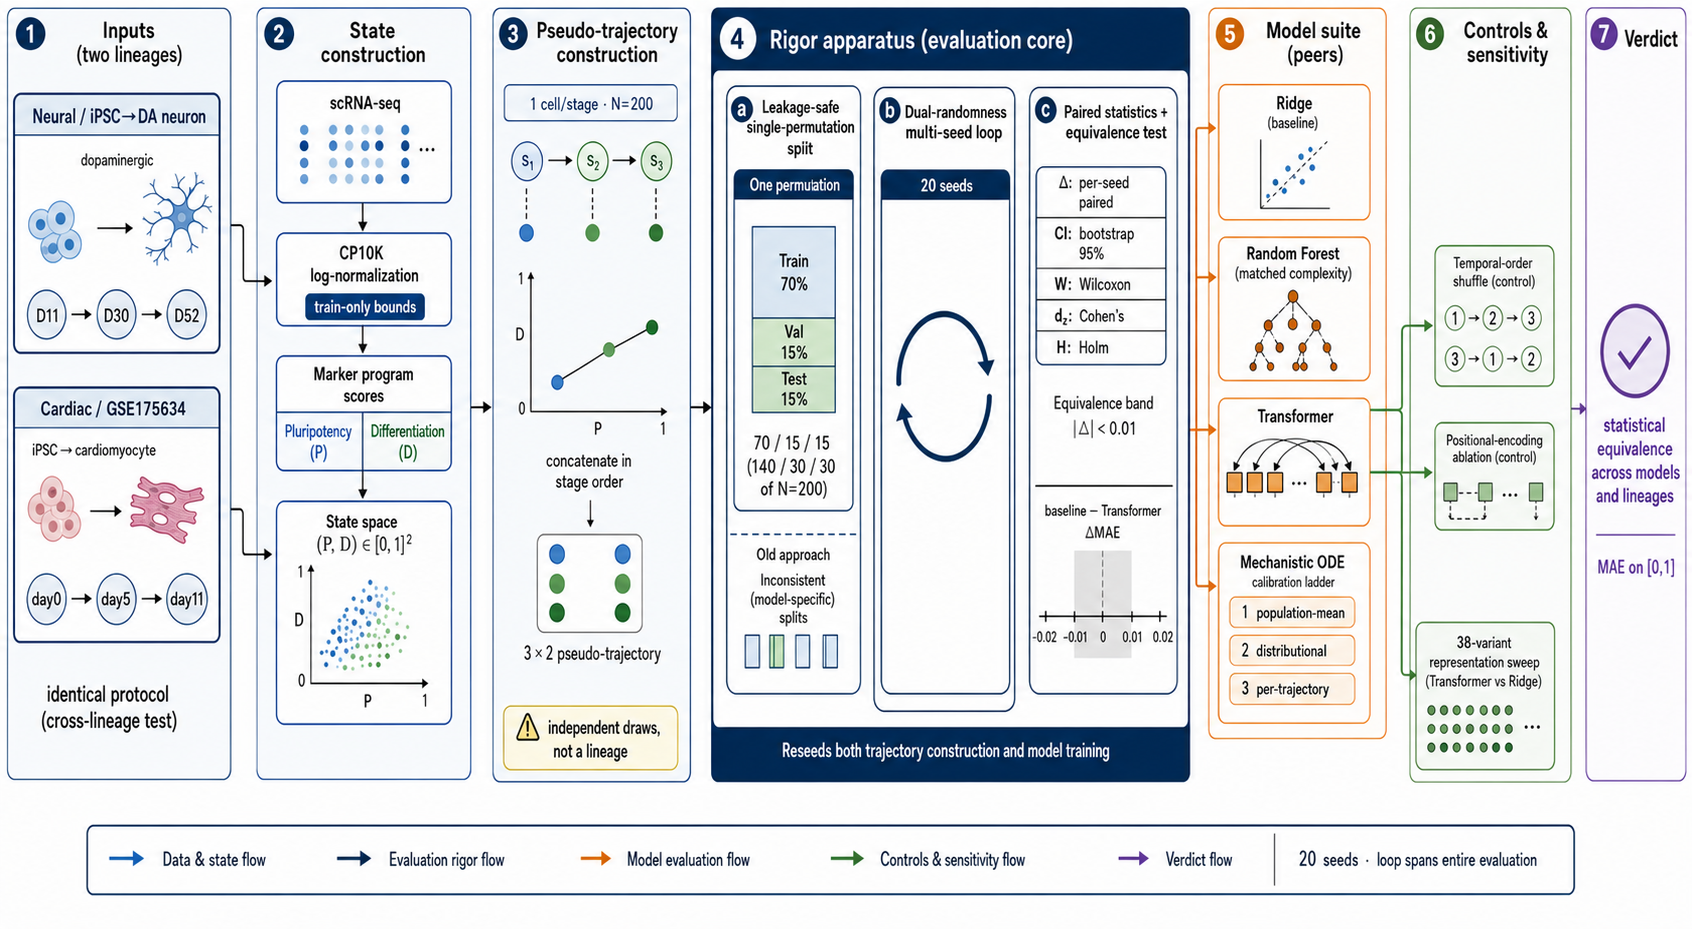
\includegraphics[width=0.99\textwidth]{figures/method_design.png}
\caption{\textbf{Overview of the leakage-safe, multi-seed, equivalence-tested forecasting benchmark.}
An identical protocol is applied to two iPSC differentiation lineages (neural, dopaminergic; cardiac, \texttt{GSE175634}), reducing scRNA-seq to a 2-D pluripotency--differentiation state and assembling stage-ordered pseudo-trajectories ($N=200$ per seed). All models share a leakage-safe $70/15/15$ split, evaluated over $20$ seeds that reseed both trajectory construction and training, and compared by paired $\Delta$MAE with bootstrap CIs, Wilcoxon tests, and an equivalence band $|\Delta|<0.01$. Four predictors (Ridge, complexity-matched random forest, Transformer, mechanistic ODE) are assessed as peers alongside temporal-order and representation controls. Arrow colors denote the data, rigor, model, control, and verdict flows.}
\label{fig:system}
\end{figure*}

The main contributions are:
\begin{itemize}
    \item An analytical null for independently paired pseudo-trajectories (Proposition~\ref{prop:null}) and its empirical confirmation on two lineages: every trained model performs no better than the constant training mean and is outperformed by the metric-matched constant training median.
    \item A leakage-safe, multi-seed, equivalence-tested evaluation protocol, with a worked example of how train--test leakage produced a spurious $19.4\%$ advantage in an earlier study.
    \item Positive controls showing that the protocol detects recoverable dependence when ground truth is known and detects the dependence a chosen coupling induces on real data, so that the null under independent pairing is attributable to the coupling rather than to the protocol, the state representation, or the sample size.
    \item Practical findings for benchmark design: the Transformer never significantly outperformed a random forest; a stage-order shuffle control is insensitive when stages are distinguishable by value; and MSE-trained models scored by MAE should be compared with the metric-matched constant.
\end{itemize}


\begin{table*}[!t]
\centering
\caption{Ways of linking cells across the time points of a differentiation time course, and what each implies for a benchmark that forecasts a late-stage state from earlier stages. The stages forecast here are separated by days to weeks, whereas labelling and velocity resolve changes over hours.}
\label{tab:rigor}
\footnotesize
\setlength{\tabcolsep}{5pt}
\renewcommand{\arraystretch}{1.1}
\begin{tabular}{>{\raggedright\arraybackslash}p{3.4cm} >{\raggedright\arraybackslash}p{5.4cm} >{\raggedright\arraybackslash}p{7.8cm}}
\toprule
\textbf{Linking strategy} & \textbf{What connects time points} & \textbf{Implication for a forecasting benchmark} \\
\midrule
Independent pairing (this study and~\cite{kanu2026transformer}) & One cell drawn independently per stage; stage order only & Late stage independent of earlier stages; the optimal forecast is a constant (Proposition~\ref{prop:null}). A \emph{null} setting by construction. \\
Pseudotime ordering~\cite{haghverdi2016diffusion,saelens2019comparison} & Cells ordered by transcriptional similarity & Orders states but does not pair a cell with its own future; imposes dependence through similarity, not lineage. \\
RNA velocity~\cite{la2018rna,bergen2020generalizing} & Spliced/unspliced ratios within a cell & Within-cell information over hours; extrapolation across gaps of days to weeks is not supported. \\
Optimal-transport couplings~\cite{schiebinger2019optimal,lavenant2024toward} & Probabilistic ancestor--descendant couplings between snapshots & Induces dependence between stages; principled under gradient-drift dynamics, but inferred, not observed. Used here as a positive control. \\
Metabolic RNA labelling~\cite{erhard2019scslam,cao2020scifate} & New vs.\ pre-existing RNA in the same cell & Observed within-cell temporal information; genuine but short-horizon. \\
Lineage barcoding~\cite{weinreb2020lineage} & Heritable barcodes shared by clonally related cells & Observed clonal coupling across days; where a forecasting advantage could be tested against ground truth. \\
\bottomrule
\end{tabular}
\end{table*}


\section{Methods}
\label{sec:methods}

Every reported quantity is an estimate with its uncertainty, computed under one protocol that is identical for all models and free of train--test leakage. Full dataset descriptions, the per-seed algorithm, model configurations, and implementation details are given in the Supplementary Material (Secs.~S1--S3 and~S8).

\subsection{Datasets and Marker Programs}
\label{subsec:data_state}

Two independent differentiation systems are analysed, so that no conclusion rests on one dataset's properties. The neural data are the population-scale iPSC$\rightarrow$dopaminergic-neuron resource of~\cite{jerber2021population}, restricted to untreated controls ($161{,}584$ cells after quality control) at day~11, 30, and 52. The cardiac data are the iPSC$\rightarrow$cardiomyocyte time course of~\cite{elorbany2022single} (\texttt{GSE175634}; $230{,}786$ cells over seven time points from more than twelve donor lines), processed from raw counts with the identical pipeline; days~0, 5, and 11 ($100{,}180$ cells) span the informative part of the trajectory before the post-day-7 plateau. Each cell is summarized by a pluripotency score $P$ and a lineage-differentiation score $D$ computed from two curated marker panels. For the neural data, $\mathcal{G}_P=\{\mathrm{POU5F1,\,NANOG,\,SOX2,\,UTF1,\,TDGF1}\}$ and $\mathcal{G}_D=\{\mathrm{TH,\,DDC,\,SLC6A3,\,DRD2,\,LMX1A,\,FOXA2}\}$; for the cardiac data, a broadened pluripotency panel (adding LIN28A and DPPA4) and a $13$-gene cardiomyocyte panel of sarcomeric, calcium-handling, and cardiac transcription-factor genes (Sec.~S1). The state recovers the expected biology---on the cardiac lineage, median $P$ falls $0.86\!\rightarrow\!0.15\!\rightarrow\!0.00$ and median $D$ rises $0.00\!\rightarrow\!0.19\!\rightarrow\!0.22$---so a null result reflects the forecasting task rather than a failure to capture differentiation.

\subsection{State Construction and Leakage-Safe Normalization}
\label{subsec:state}

Counts are library-size normalized to $10{,}000$ per cell and log-transformed, and the raw scores are panel means, $P^{\mathrm{raw}}_t=|\mathcal{G}_P|^{-1}\sum_{g\in\mathcal{G}_P}\log(1+\mathrm{expr}_t(g))$ and likewise for $D^{\mathrm{raw}}_t$. Each raw score is min--max scaled using bounds from the training partition only, then clipped:
\begin{equation}
z^{\mathrm{norm}} = \mathrm{clip}\!\left(\frac{z - z_{\min}^{\mathrm{tr}}}{z_{\max}^{\mathrm{tr}} - z_{\min}^{\mathrm{tr}}},\;0,\;1\right), \quad z\in\{P^{\mathrm{raw}},D^{\mathrm{raw}}\},
\label{eq:minmax_clip}
\end{equation}
giving the stage state $s_t=[P_t,D_t]\in[0,1]^2$. Estimating bounds on the full dataset, a common shortcut, would let the held-out range influence preprocessing. Clipping places many late-stage values exactly at the lower bound, because marker panels are often undetected in individual cells: on average, $50\%$ (neural) and $83\%$ (cardiac) of late-stage training $P$ values and $36\%$ and $28\%$ of $D$ values equal zero. The late-stage marginals are therefore strongly skewed, and their mean and median differ markedly, which matters for the constant baseline (Sec.~\ref{subsec:res_constant}).

\subsection{Pseudo-Trajectory Construction and Its Encoded Assumption}
\label{subsec:traj}

Because the datasets do not link the same cell across stages, sequences are assembled by sampling one cell independently (with replacement) per stage and concatenating their states in stage order:
\begin{equation}
x^{(i)}=\big[s_{t_0}^{(i)},\,s_{t_1}^{(i)},\,s_{t_2}^{(i)}\big],
\qquad i=1,\dots,N,\;\; N=200.
\label{eq:traj_def}
\end{equation}
Each $x^{(i)}$ is a \emph{population-level pseudo-trajectory}, not a tracked lineage: its three states are independent draws from the stage marginals, and the target $s_{t_2}$ is not the future state of any individual cell. This construction is retained because it mirrors the original study~\cite{kanu2026transformer} and many comparable analyses. Algorithm~S1 gives the per-seed procedure. The independence has a direct consequence.

\begin{proposition}[Independent pairing implies a constant optimal predictor]
\label{prop:null}
Let a test pseudo-trajectory be generated by Eq.~\eqref{eq:traj_def}, so that $s_{t_2}$ is independent of $x=(s_{t_0},s_{t_1})$, and let $f$ be any predictor fitted on training trajectories drawn independently of that test trajectory. Let $m=(m_P,m_D)$ be the component-wise median of the marginal distribution of $s_{t_2}$. Then
\[
\mathbb{E}\big[\mathrm{MAE}_s(f)\big]\;\ge\;\mathbb{E}\big[\mathrm{MAE}_s(m)\big],
\]
with equality only if $f(x)$ is a component-wise median of $s_{t_2}$ for almost every $x$. In particular, $\mathbb{E}[s_{t_2}\mid x]=\mathbb{E}[s_{t_2}]$, and the Bayes-optimal predictor under absolute loss is the constant $m$.
\end{proposition}

\noindent\emph{Proof.} Condition on $x$ and on the training data. The prediction $c=f(x)$ is then fixed, and because $s_{t_2}$ is independent of both, $\mathbb{E}\,|s_{t_2,k}-c_k|$ is minimized, for each component $k\in\{P,D\}$, by any median of the marginal of $s_{t_2,k}$. Averaging over $x$ and the training data gives the inequality. $\square$

Proposition~\ref{prop:null} makes three predictions before any model is trained: (i)~no model can outperform the constant marginal median in expectation, so models of any capacity can at best tie; (ii)~input transformations such as permuting stage order or removing positional encoding cannot change attainable accuracy; and (iii)~input-dependent flexibility, including per-trajectory calibration of a dynamical model, can only add variance. The analyses below test whether the protocol recovers this known null and whether a protocol lacking its safeguards would report a spurious advantage (Sec.~\ref{subsec:res_leakage}); the positive controls (Sec.~\ref{subsec:positive}) test behaviour when genuine dependence is present.

\subsection{Multi-Seed Evaluation Protocol and Statistics}
\label{subsec:protocol}

The task maps the two earliest states to the latest, $\hat{s}_{t_2}=f(s_{t_0},s_{t_1})$, scored by $\mathrm{MAE}_s=\tfrac{1}{2}(\mathrm{MAE}_P+\mathrm{MAE}_D)$, the mean absolute error averaged over the two state components. Because trajectory construction and training are both stochastic, a single seed yields one realization whose variability is unknown; MAE is therefore treated as a random variable. The protocol runs $S=20$ seeds, each perturbing \emph{both} pseudo-trajectory construction (which cells are sampled, paired, and split) and model training (weight initialization, dropout, minibatch order, and bootstrap resampling). Within each seed, the $N=200$ trajectory indices are permuted once and partitioned $70/15/15$ ($140/30/30$); the resulting disjoint index sets are shared identically by every model, so that each between-model difference on a seed is a genuine paired observation and no trajectory appears in more than one partition.

Each baseline is compared to the Transformer via the per-seed paired difference $\Delta^{(s)} = \mathrm{MAE}^{(s)}_{\text{baseline}} - \mathrm{MAE}^{(s)}_{\text{Transformer}}$, summarized by a percentile paired-bootstrap $95\%$ CI on $\overline{\Delta}$ ($10^4$ resamples), a Wilcoxon signed-rank test, and the effect size $d_z=\overline{\Delta}/\mathrm{sd}(\Delta)$, with Holm--Bonferroni correction across baselines. Following the two-one-sided-tests logic~\cite{lakens2017equivalence}, two models are declared \emph{equivalent} only when the entire $95\%$ CI on $\overline{\Delta}$ lies within $|\Delta|<\delta=0.01$ MAE units, about $6\%$ (neural) and $9\%$ (cardiac) of the Ridge MAE and half the seed-to-seed standard deviation. The margin was fixed in the original analysis code but not preregistered, so the equivalence analysis is best read as a sensitivity criterion; all equivalence conclusions hold at any margin of at least $0.0093$ (Sec.~S4). A CI that merely contains zero is \emph{not} taken as evidence of equivalence.

\subsection{Predictive Models}
\label{subsec:models}

\emph{Constant baselines.} The constant training-median predictor returns $(m_P,m_D)$, the per-seed medians of the normalized late-stage training targets, for every test trajectory. It is the training-sample estimate of $m$ in Proposition~\ref{prop:null}, and hence the reference against which every model is judged. The constant training mean, the input-independent optimum of the squared-error loss used to train the other models, is scored as a diagnostic. Both are computed on exactly the per-seed trajectories and splits of the other models (Sec.~S3).

\emph{Ridge and random forest.} Both operate on the flattened context $x=[P_{t_0},D_{t_0},P_{t_1},D_{t_1}]\in\mathbb{R}^4$. Ridge regression ($\alpha=1$; ten parameters) is the simplest model that can express a dependence of the late state on the early states. The random forest tests whether nonlinear capacity \emph{without} sequence structure helps; it is complexity-matched by per-seed 3-fold cross-validation over depth and leaf size on the training partition.

\emph{Transformer.} The encoder treats $[s_{t_0},s_{t_1}]$ as a length-two token sequence with a sinusoidal positional encoding (4 layers, 8 heads, $d_{\mathrm{model}}=128$, $\approx$827K parameters; MSE loss, best-validation selection; Sec.~S3). The positional encoding and self-attention over the two stages are the only routes by which temporal order enters, and Sec.~\ref{subsec:controls} tests exactly these.

\emph{Mechanistic ODE.} A phenomenological two-state model, benchmarked against the Transformer in the original study~\cite{kanu2026transformer}, encodes the hypothesis that pluripotency is lost while differentiation is induced through a $P$--$D$ commitment interaction:
\begin{align}
\frac{dP}{dt} &= k_{ps}(1-P) - k_{pd}P - rPD,
\label{eq:ode_p}\\
\frac{dD}{dt} &= k_b + k_{ds}PD + rPD - k_{dd}D,
\label{eq:ode_d}
\end{align}
integrated over the calendar-time intervals between stages, with $k_{ps}$ and $k_{dd}$ fixed and four rates free. To separate whether the ODE \emph{can} fit the data from whether fitting it more faithfully \emph{helps}, the free rates are calibrated by differential evolution under three regimes of increasing sample-level fidelity: to the population-mean trajectory; to the training distribution's mean and standard deviation; and per test trajectory to its own $t_0\!\rightarrow\!t_1$ step (Sec.~S3).
\label{subsec:ode_calib}

\subsection{Temporal and Representation Controls}
\label{subsec:controls}

Whether the Transformer uses temporal structure is measured, not assumed. The \emph{stage-order shuffle} randomly swaps the two input tokens of each trajectory (probability $1/2$, applied identically to all partitions; the target is never moved), destroying consistent ordering while preserving stage values. The \emph{positional-encoding ablation} removes $\mathrm{PE}(t)$ while leaving capacity intact. Both are compared to the ordered model across all $20$ seeds and reported as equivalence statements. When stages differ systematically in value, a model can identify the earlier input from the values themselves, so an unchanged error under shuffling does not by itself show that the data lack temporal dependence; the positive controls quantify this limitation.
\label{subsec:sensitivity}
To ensure that no conclusion depends on the particular 2D state, the Transformer-versus-Ridge gap is also recomputed, with $20$ seeds each, across $38$ state-construction variants: leave-one-marker-out for every panel gene, per-gene median and $z$-score aggregation instead of the mean of logs, and an enlarged neural panel ($15$ neural and $23$ cardiac variants). The same sampled cells are reused across variants within a seed.

\subsection{Positive Controls: Settings With Temporal Dependence}
\label{subsec:positive}

A protocol that always reports no advantage would also pass the test of Proposition~\ref{prop:null}. Two positive controls therefore ask whether the identical protocol detects temporal dependence when pseudo-trajectories carry it. Both are run at $N=200$ ($20$ seeds) and at $N=2{,}000$ ($10$ seeds), to test whether conclusions depend on sample size.

\subsubsection{Simulated differentiation with a known coupling} Cell states $X=(P,D)$ follow the gradient stochastic differential equation
\begin{equation}
\begin{aligned}
dX_t&=-\nabla V(X_t)\,dt+\sigma\,dW_t,\\
V(P,D)&=\tfrac{a}{2}P^2+b\,(D-d_{\mathrm{lo}})^2(D-d_{\mathrm{hi}})^2,
\end{aligned}
\label{eq:sde}
\end{equation}
observed at $t=0,1,2$: pluripotency decays while each cell commits from near the barrier of a double well to a low- or high-differentiation fate, so the late state depends on the early states. Each stage is observed in an independent snapshot population, mirroring destructive measurement. Three constructions are compared: \emph{true} trajectories of tracked particles (an oracle unavailable in real data); \emph{independent} pairing of snapshot cells; and \emph{OT-coupled} trajectories sampled as a Markov chain along entropic optimal-transport plans between consecutive snapshots, the standard way of chaining OT couplings~\cite{schiebinger2019optimal} with heat-kernel regularization~\cite{lavenant2024toward} (Sec.~S5). Every model is scored on its own test split and on held-out true trajectories.

\subsubsection{OT-coupled pseudo-trajectories from the real data} For each lineage, OT couplings between consecutive stages are computed in a $30$-component PCA embedding of $2{,}000$ highly variable genes, rather than in $(P,D)$ space, so that the induced dependence is not built from the target variables; trajectories are sampled along the chain as above (Sec.~S5). The same cells also yield independently paired trajectories, so the two constructions differ only in the coupling. No ground truth exists here: an advantage under OT coupling shows that the protocol detects the dependence the coupling induces, not that this dependence is biological.

\subsection{Implementation and Reproducibility}
\label{subsec:impl_repro}

All preprocessing and trajectory construction are seeded and serialized, and every figure and table value is generated programmatically from per-seed outputs; no reported number is entered by hand. This is the mechanism by which the leakage that affected the original analysis~\cite{kanu2026transformer} was detected and prevented from recurring. The software stack is listed in Table~S1.


\section{Results}
\label{sec:results}

\subsection{On Independently Paired Data, the Transformer Matches Both Baselines}
\label{subsec:res_neural}

Repeating the full pipeline over $20$ seeds yields the distributions in Fig.~\ref{fig:raincloud}A and the paired comparisons in Fig.~\ref{fig:forest} (neural). All three models occupy the same MAE range: Ridge $0.1774\pm0.0204$, the complexity-matched random forest $0.1794\pm0.0208$, and the Transformer $0.1787\pm0.0203$ (mean\,$\pm$\,s.d.\ over seeds). The paired differences against the Transformer are negligible---Ridge $\overline{\Delta}=-0.0013$ ($d_z=-0.14$, $p=0.996$) and random forest $\overline{\Delta}=+0.0007$ ($d_z=+0.07$, $p=0.996$, Holm-corrected)---with $95\%$ CIs contained within the equivalence margin, supporting equivalence rather than merely failing to reject a difference. The seed-to-seed spread (s.d.\ $\approx 0.020$) is an order of magnitude larger than any between-model mean difference ($\le 0.0013$), which is why a single-seed comparison could report a spurious ranking: the gap was smaller than the noise it was drawn from.

\begin{figure}[!t]
\centering
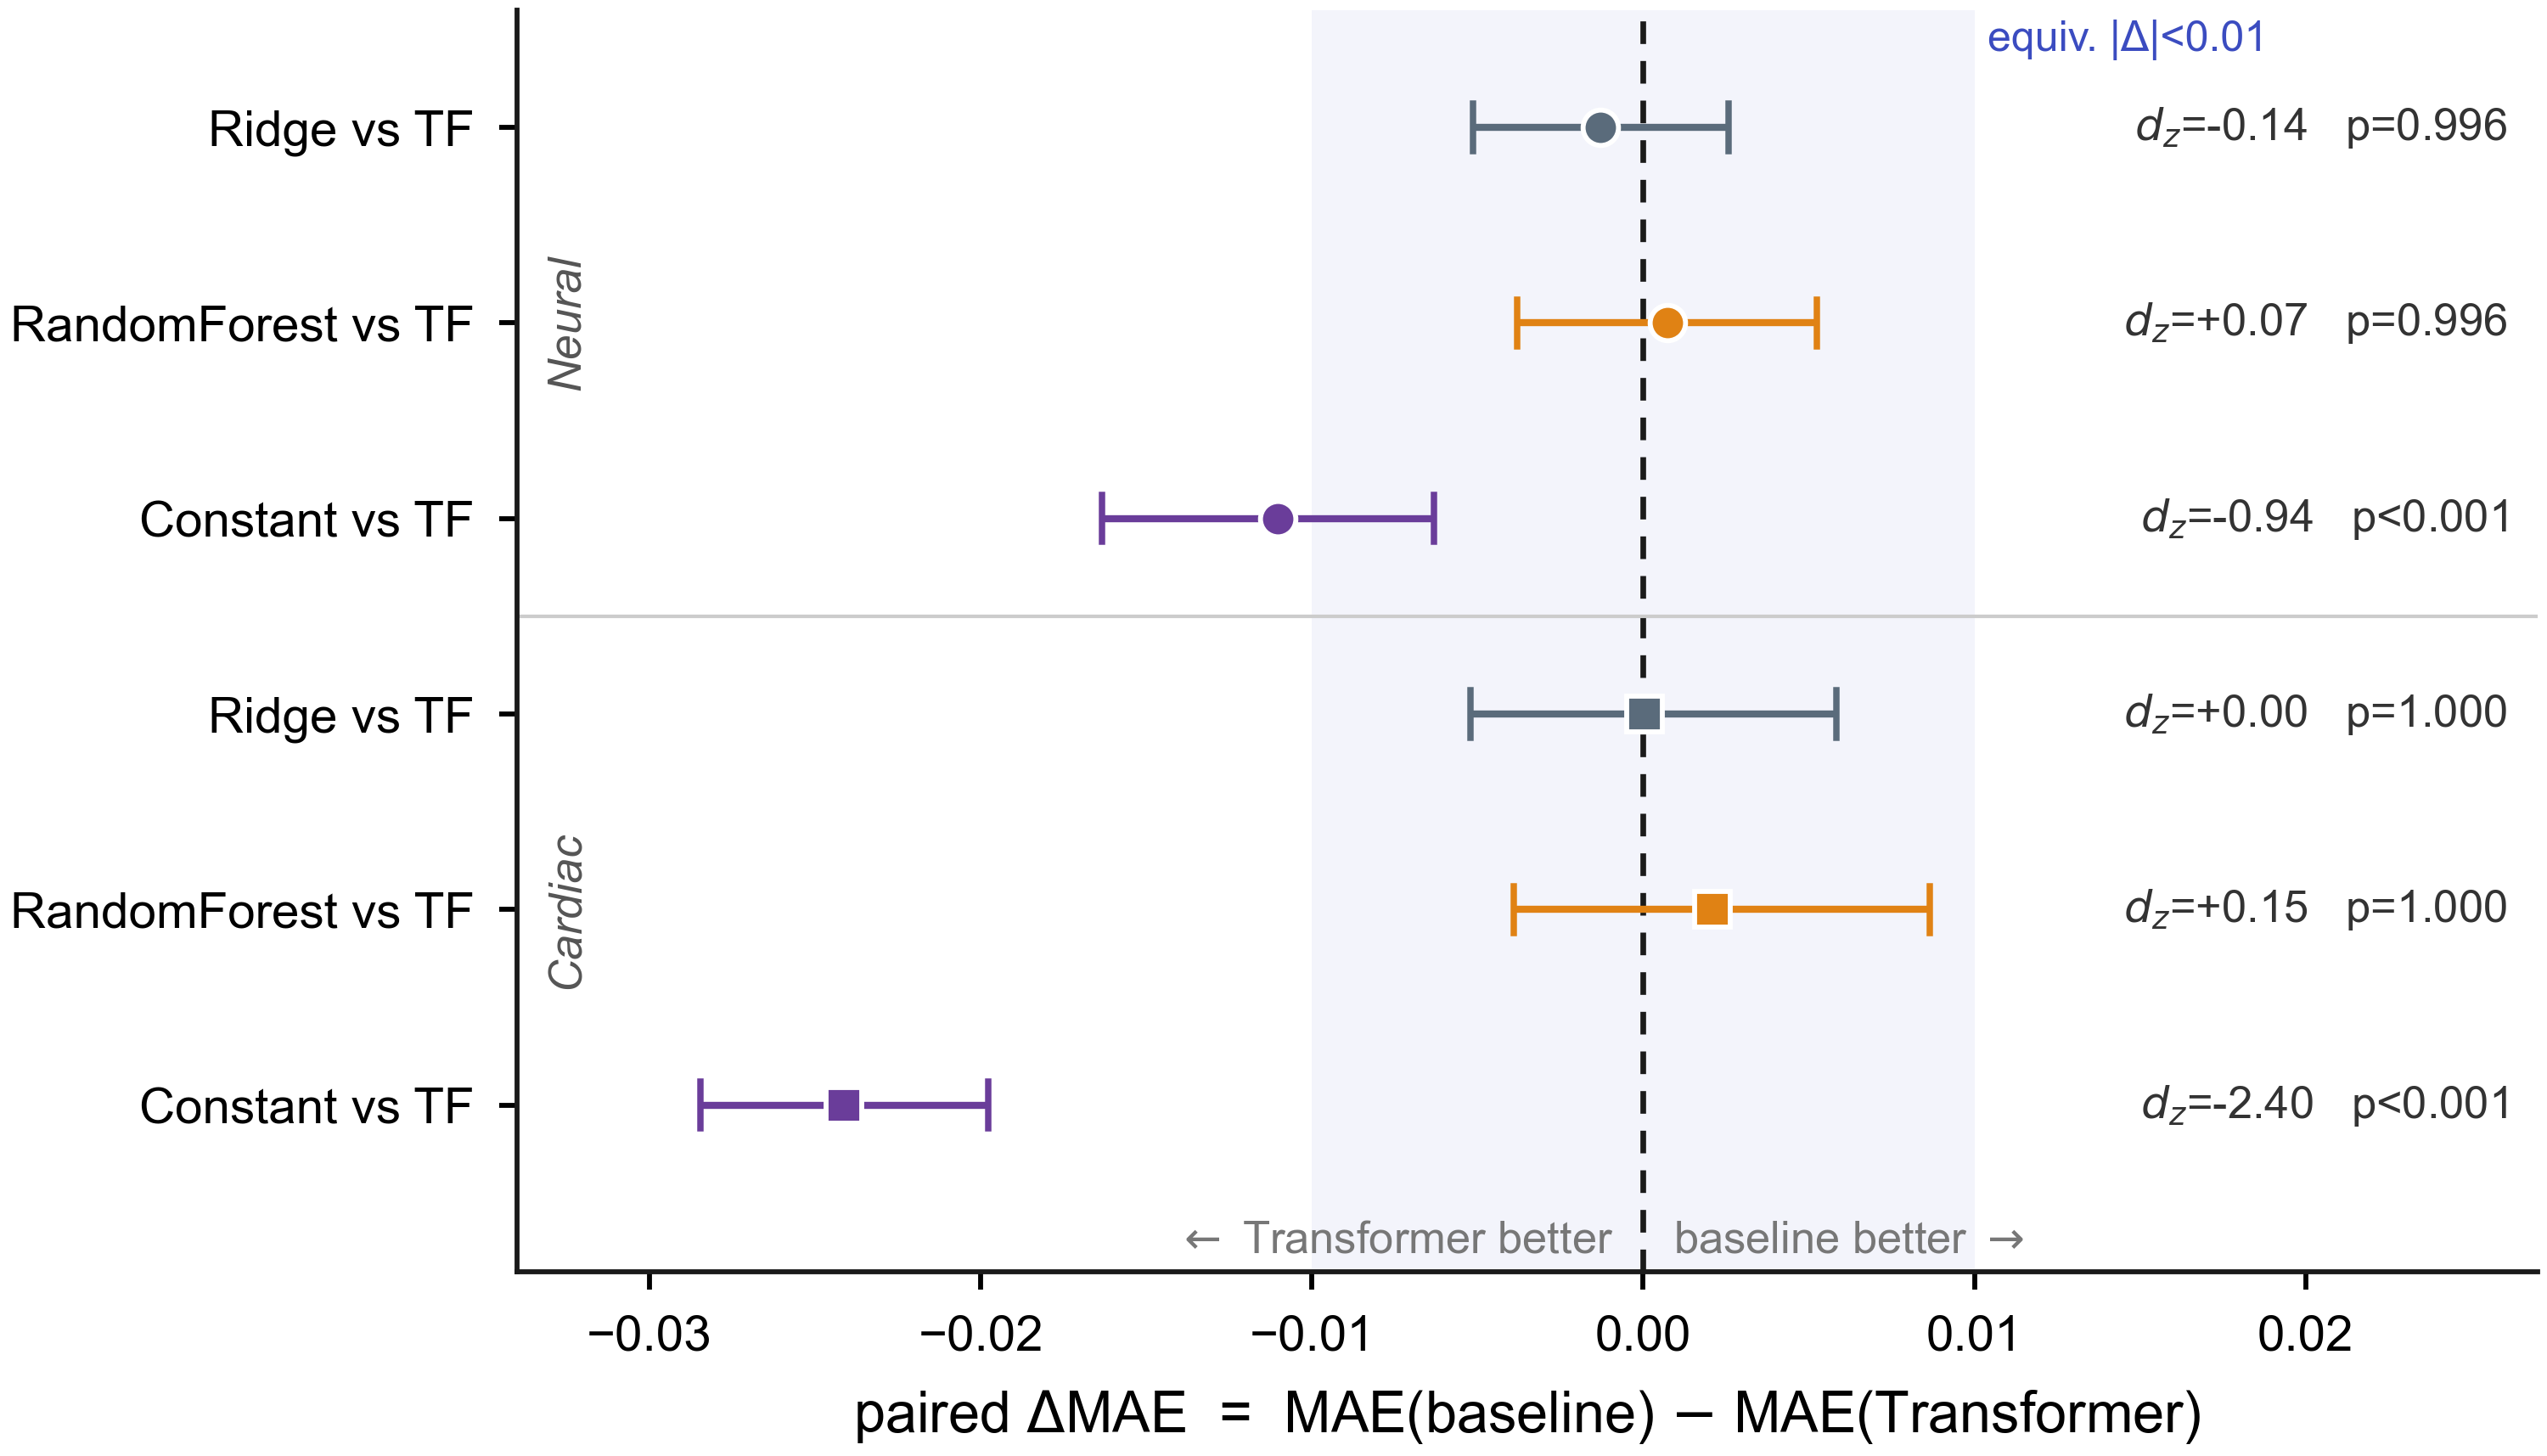
\includegraphics[width=\columnwidth]{figures/fig2_forest.png}
\caption{\textbf{The trained models are equivalent to one another, and all are beaten by a constant.} Paired difference $\Delta=\mathrm{MAE}_{\text{baseline}}-\mathrm{MAE}_{\text{Transformer}}$ ($n=20$ seeds) with percentile paired-bootstrap $95\%$ CIs; positive values favour the Transformer's competitors. Annotations give Cohen's $d_z$ and Holm-corrected Wilcoxon $p$. Shaded band, equivalence region $|\Delta|<0.01$. Ridge and the random forest lie within the band on both lineages; the constant training median (purple) is significantly better than the Transformer on both.}
\label{fig:forest}
\end{figure}

\subsection{The Equivalence Replicates on an Independent Cardiac Lineage}
\label{subsec:res_cardiac}

On the cardiac lineage the equivalence replicates exactly (Fig.~\ref{fig:raincloud}B, Fig.~\ref{fig:forest}): Ridge $0.1100\pm0.0155$, random forest $0.1121\pm0.0175$, and Transformer $0.1100\pm0.0198$, with paired differences against the Transformer of $\overline{\Delta}\approx0$ for Ridge ($p=1.000$) and $+0.0021$ for the random forest ($d_z=+0.15$, $p=1.000$), both within the margin. Across two lineages and $40$ seeds, no trained model significantly outperforms the linear baseline.

\subsection{A Constant Predictor Outperforms Every Trained Model}
\label{subsec:res_constant}

Proposition~\ref{prop:null} predicts that no model can beat the constant training median. Scoring that constant on the identical per-seed splits confirms the prediction and goes further: the constant is significantly \emph{better} than every trained model on both lineages (Table~\ref{tab:constant}). On the cardiac lineage it has lower error than every model on all $20$ seeds, by $0.024$--$0.026$ MAE ($28$--$31\%$ of its error; $d_z=2.4$--$3.9$; Holm-corrected $p<10^{-5}$); on the neural lineage it is better on $17$ of $20$ seeds, by $0.010$--$0.012$ ($6$--$7\%$; $d_z=0.77$--$0.94$; $p<0.005$).

The gap is explained by the loss functions rather than by overfitting. The trained models minimize squared error, whose input-independent optimum is the training \emph{mean}; scored as a constant, that mean reaches $0.1762$ (neural) and $0.1091$ (cardiac), essentially the MAE of every trained model. The trained models thus behave as approximately input-independent predictors (test MAE alone does not show that their predictions are exactly constant). Under absolute error the median is optimal instead, and because the late-stage marginals are skewed by mass at the lower bound (Sec.~\ref{subsec:state}), mean and median differ substantially. The ranking among trained models therefore carries no information about temporal modelling.

\begin{figure*}[!t]
\centering
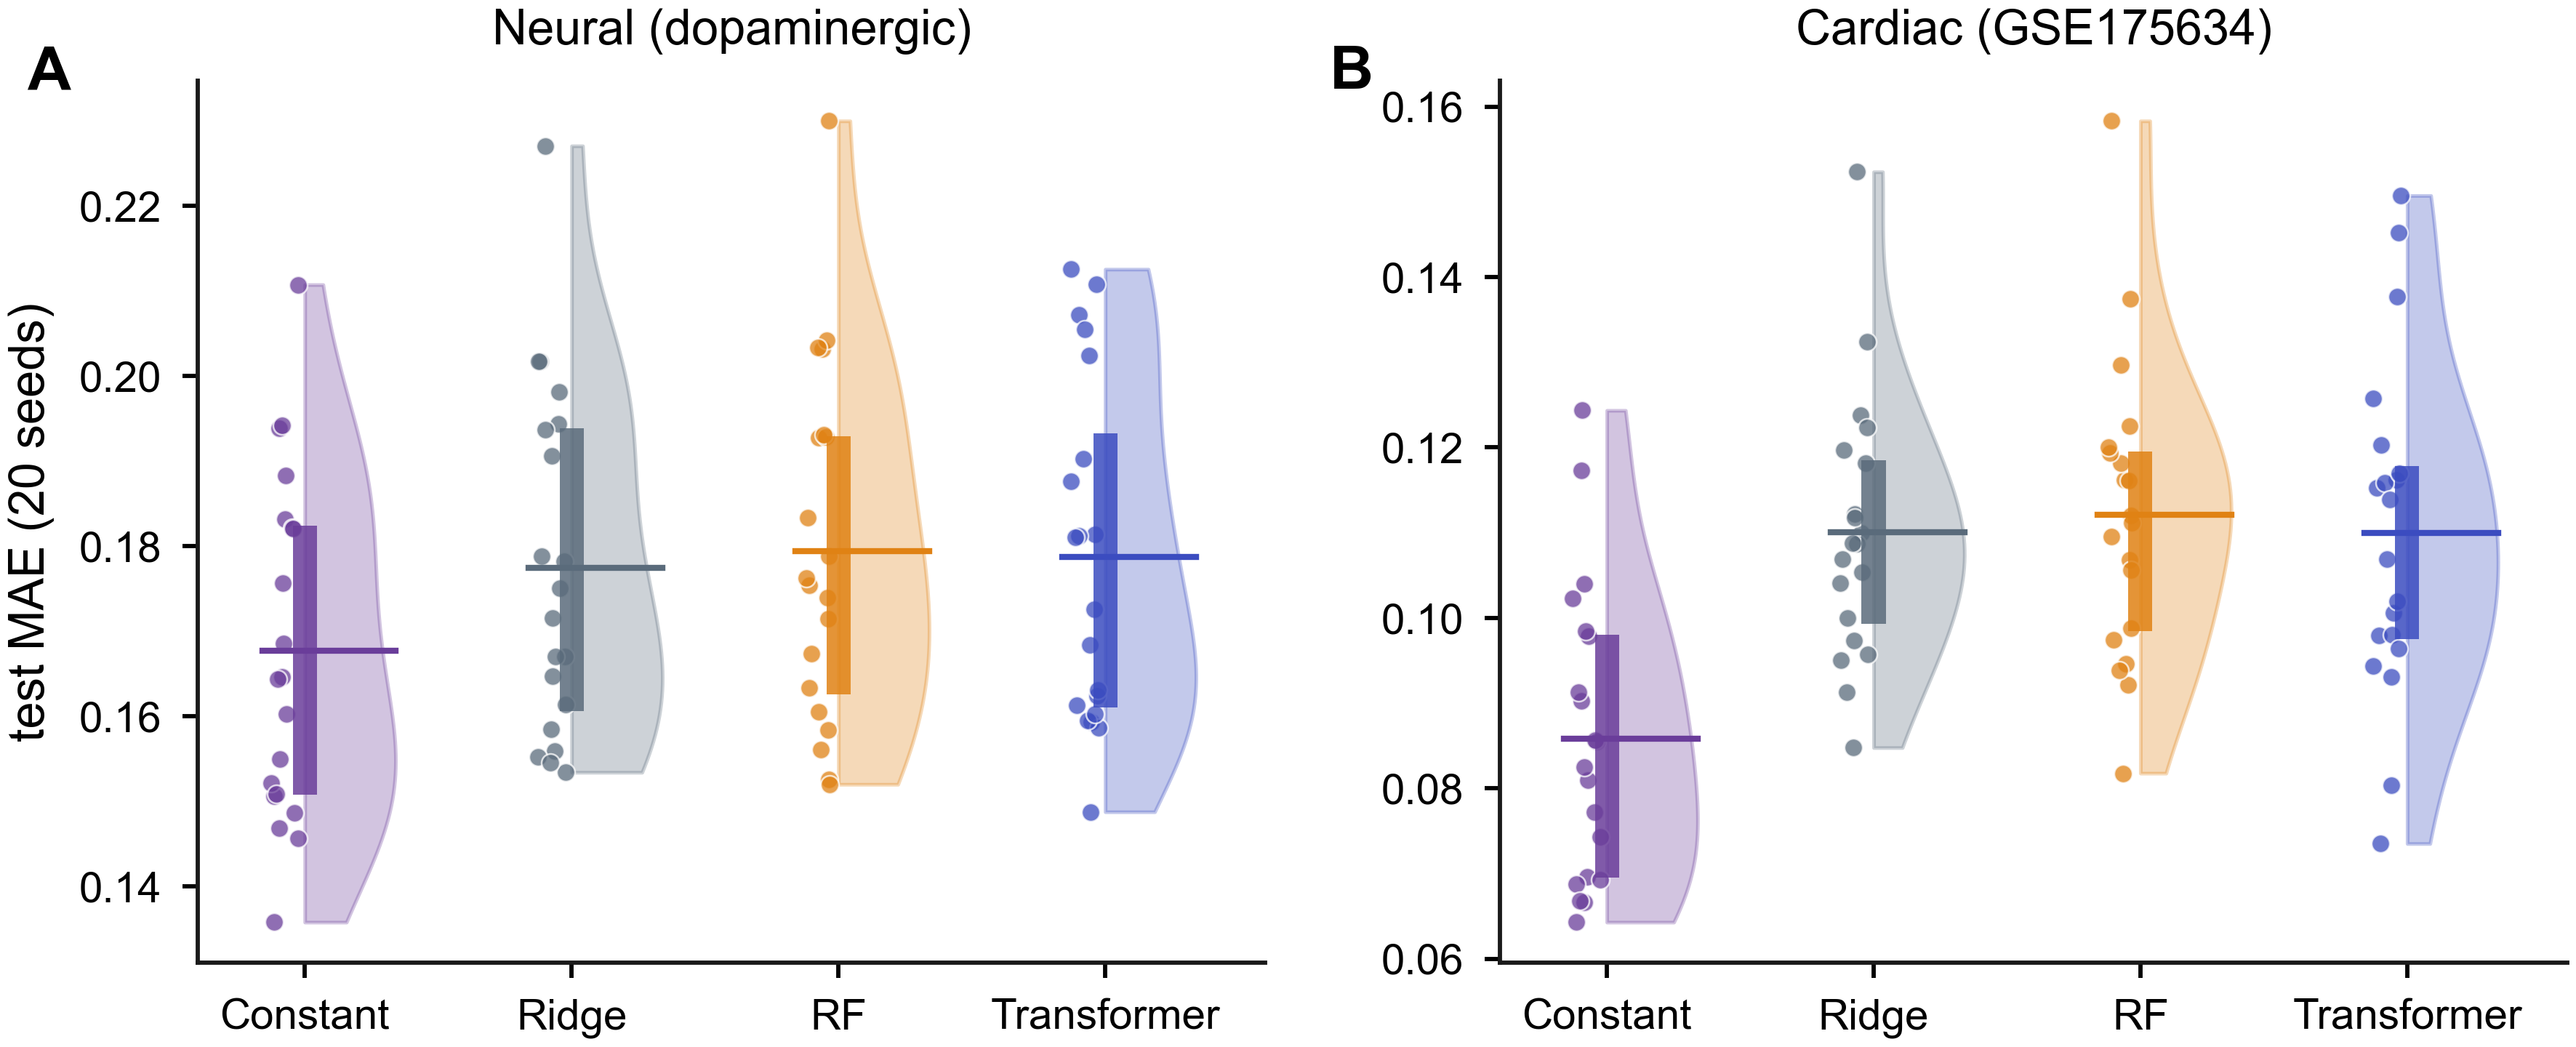
\includegraphics[width=0.84\textwidth]{figures/fig3_raincloud.png}
\caption{\textbf{The trained models' error distributions are superimposed; the constant's sits lower.} Test MAE over $n=20$ seeds for the constant training median, Ridge, the complexity-matched random forest, and the Transformer on the neural \textbf{(A)} and cardiac \textbf{(B)} lineages, shown as half-violin density, jittered per-seed points, and per-model mean (horizontal line). The seed-to-seed spread (s.d.\ $\approx0.020$ neural, $\approx0.017$ cardiac) dwarfs every between-model mean difference ($\le0.0021$), so a single-seed comparison cannot resolve a reliable ranking.}
\label{fig:raincloud}
\end{figure*}

\begin{table}[!t]
\centering
\caption{Mean test MAE over $20$ seeds and paired difference $\overline{\Delta}=\mathrm{MAE}_{\text{model}}-\mathrm{MAE}_{\text{constant}}$ against the constant training median, with percentile paired-bootstrap $95\%$ CI. Positive values favour the constant; all differences are significant (Wilcoxon, Holm-corrected $p<0.005$).}
\label{tab:constant}
\footnotesize
\setlength{\tabcolsep}{1.8pt}
\begin{tabular}{lcccc}
\toprule
 & \multicolumn{2}{c}{\textbf{Neural}} & \multicolumn{2}{c}{\textbf{Cardiac}} \\
\cmidrule(lr){2-3}\cmidrule(lr){4-5}
\textbf{Predictor} & \textbf{MAE} & $\overline{\Delta}$ [95\% CI] & \textbf{MAE} & $\overline{\Delta}$ [95\% CI] \\
\midrule
Const.\ (median) & $.1677$ & --- & $.0859$ & --- \\
Const.\ (mean) & $.1762$ & --- & $.1091$ & --- \\
Ridge & $.1774$ & $.0098$ [$.0042$, $.0149$] & $.1100$ & $.0242$ [$.0217$, $.0270$] \\
Random forest & $.1794$ & $.0118$ [$.0061$, $.0172$] & $.1121$ & $.0262$ [$.0232$, $.0297$] \\
Transformer & $.1787$ & $.0110$ [$.0063$, $.0163$] & $.1100$ & $.0241$ [$.0198$, $.0285$] \\
\bottomrule
\end{tabular}
\end{table}

\subsection{Temporal, Mechanistic, and Representation Controls Are Consistent With the Null}
\label{subsec:res_temporal}
\label{subsec:res_ode}
\label{subsec:res_sensitivity}

Permuting the input stage order or removing the positional encoding leaves the Transformer's test MAE unchanged on both lineages (Fig.~S1): shuffle-vs-ordered $\overline{\Delta}=-0.0002$ on the neural ($p=0.87$) and cardiac ($p=0.90$) lineages, $1$--$3\%$ of the seed-to-seed standard deviation, with the no-PE ablation equally inert. This is consistent with Proposition~\ref{prop:null} but, on its own, weak evidence: the positive control (Sec.~\ref{subsec:res_positive}) shows that the shuffle is insensitive even when strong dependence is present.

The mechanistic ODE degrades monotonically as its calibration is made fairer (Fig.~\ref{fig:ode}). On the neural lineage its test MAE rises from $0.198$ (population-mean; $+12\%$ over Ridge) through $0.295$ (distributional; $+66\%$) to $0.370$ (per-trajectory; $+108\%$); on the cardiac lineage from $0.248$ ($+126\%$) through $0.258$ ($+135\%$) to $0.334$ ($+203\%$). Because the early step of an independently paired trajectory carries no information about its late state, added freedom to fit it fits noise, exactly as Proposition~\ref{prop:null} predicts. This is a statement about population-level priors on pseudo-trajectory data, not a general verdict on mechanistic modelling.

Across the $38$ state-construction variants, the paired Transformer$-$Ridge gap is centred near zero (mean $+0.0004$, range $[-0.0016,+0.0028]$, maximum $|d_z|=0.19$), every interval lies within the equivalence margin, and \emph{no} variant produces a significant Transformer advantage ($0/38$; Fig.~\ref{fig:sensitivity}). The conclusion is a property of the task, not of a specific feature definition.

\begin{figure}[!t]
\centering
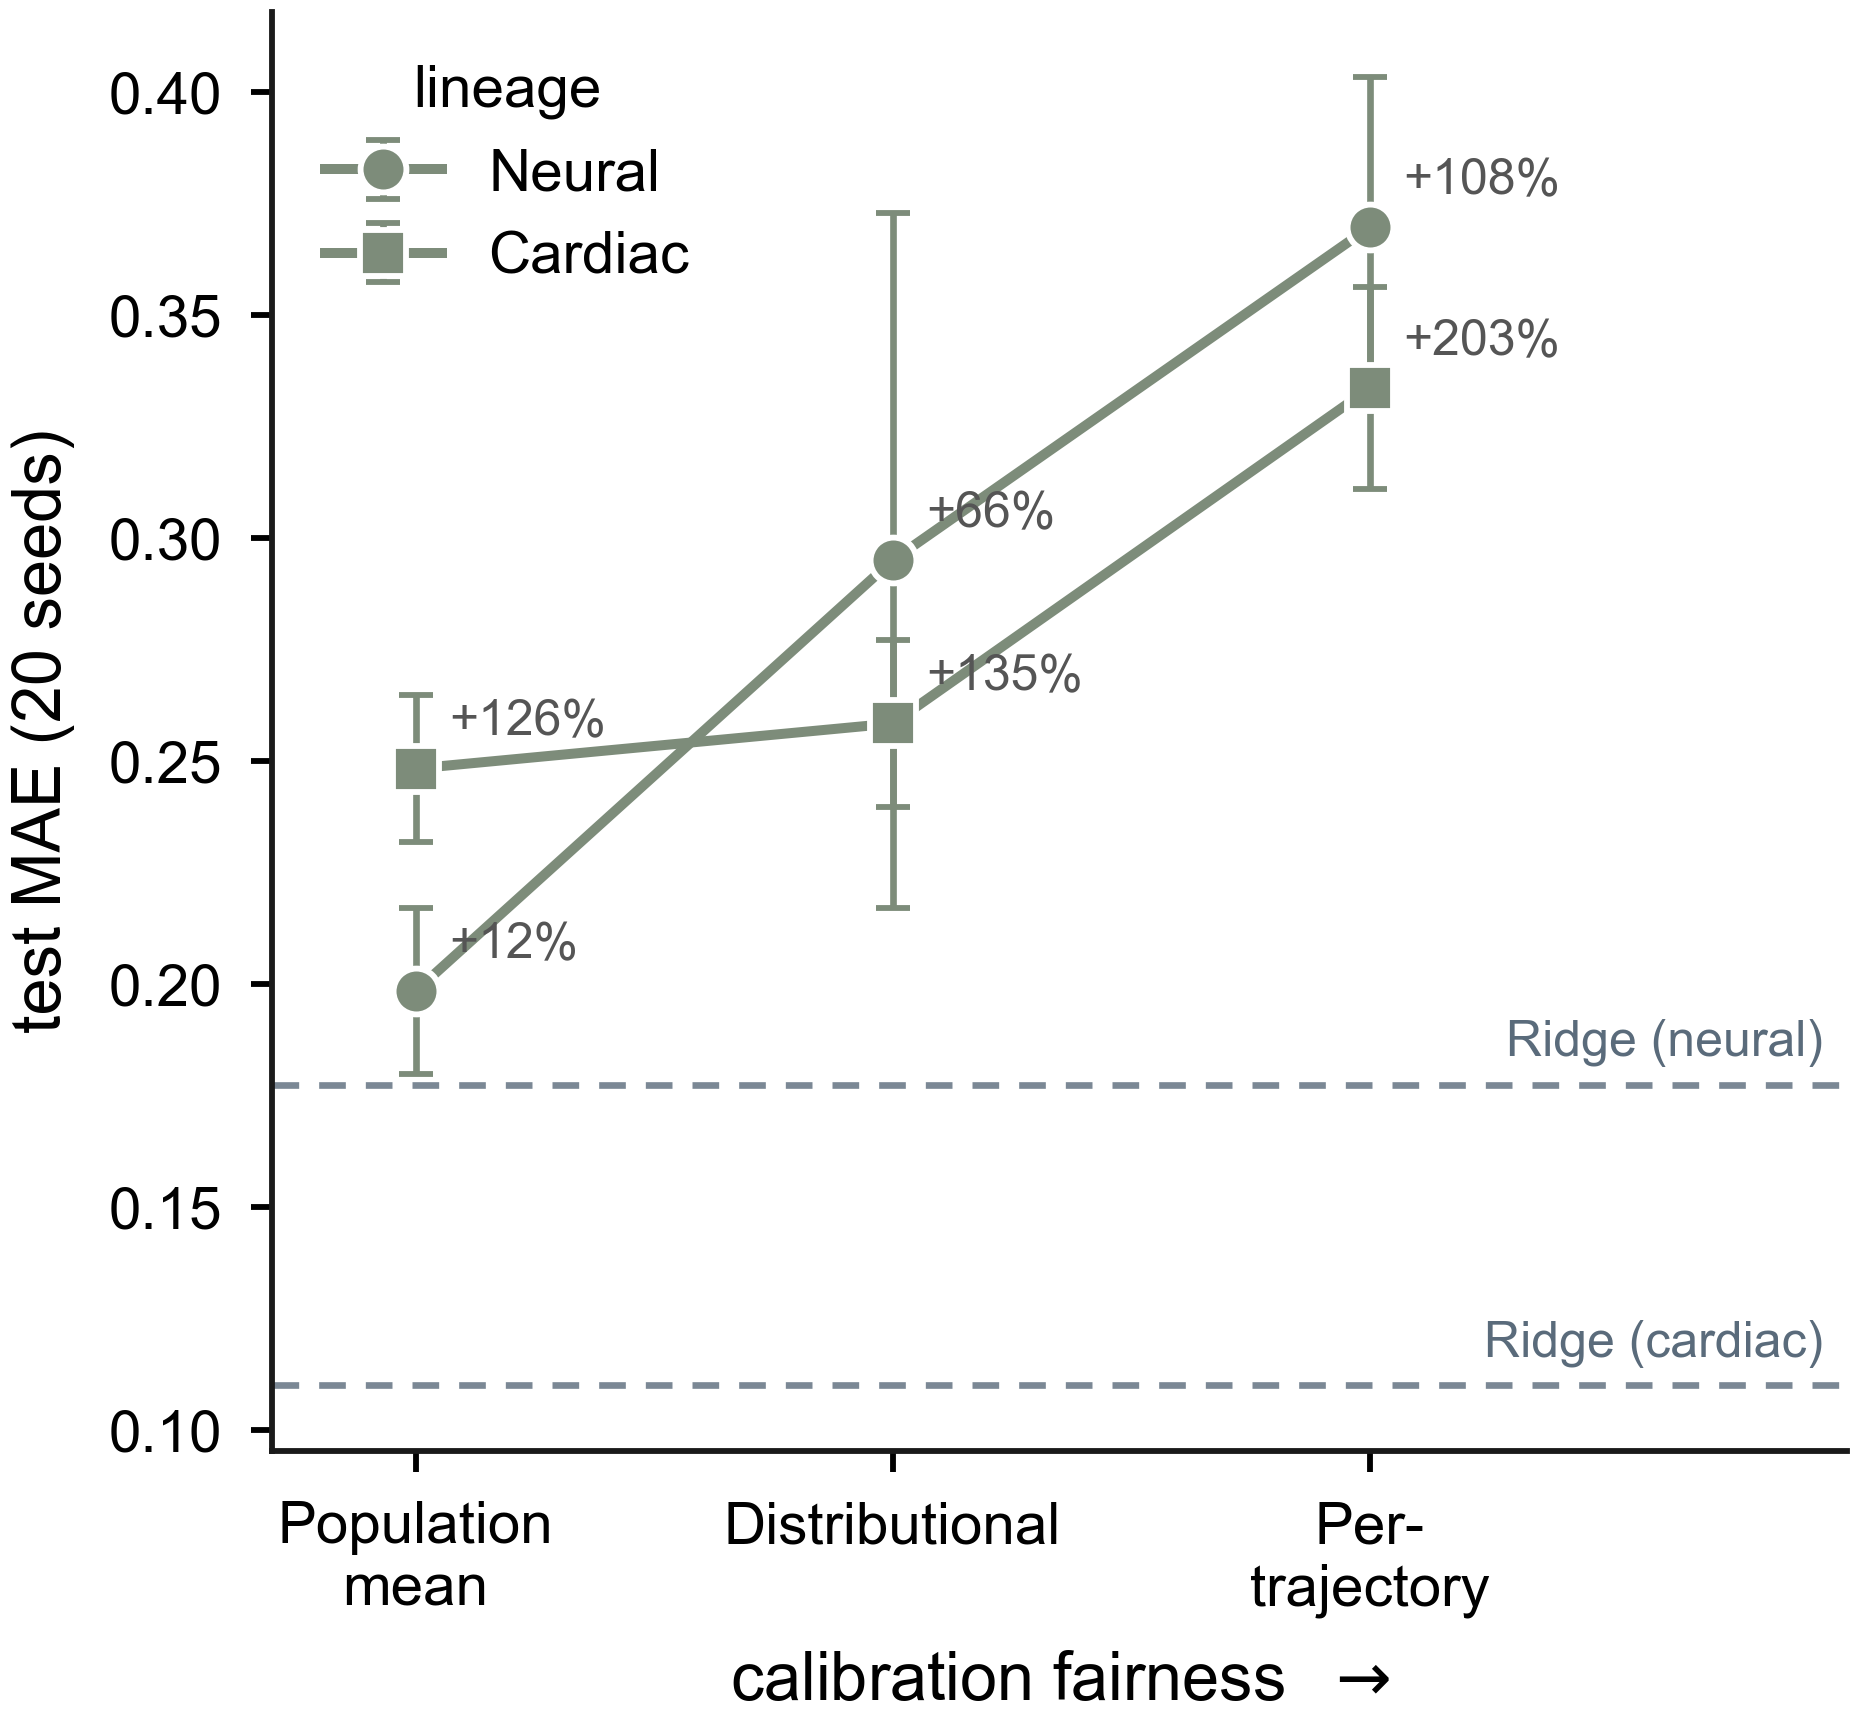
\includegraphics[width=\columnwidth]{figures/fig5_ode.png}
\caption{\textbf{Fairer sample-level calibration of the mechanistic model worsens prediction.} Test MAE ($n=20$ seeds, mean with s.d.\ whiskers) of the mechanistic ODE under three calibration regimes of increasing sample-level fidelity, for the neural (circles) and cardiac (squares) lineages; annotations give the increase over the corresponding Ridge baseline (dashed references).}
\label{fig:ode}
\end{figure}

\begin{figure}[!t]
\centering
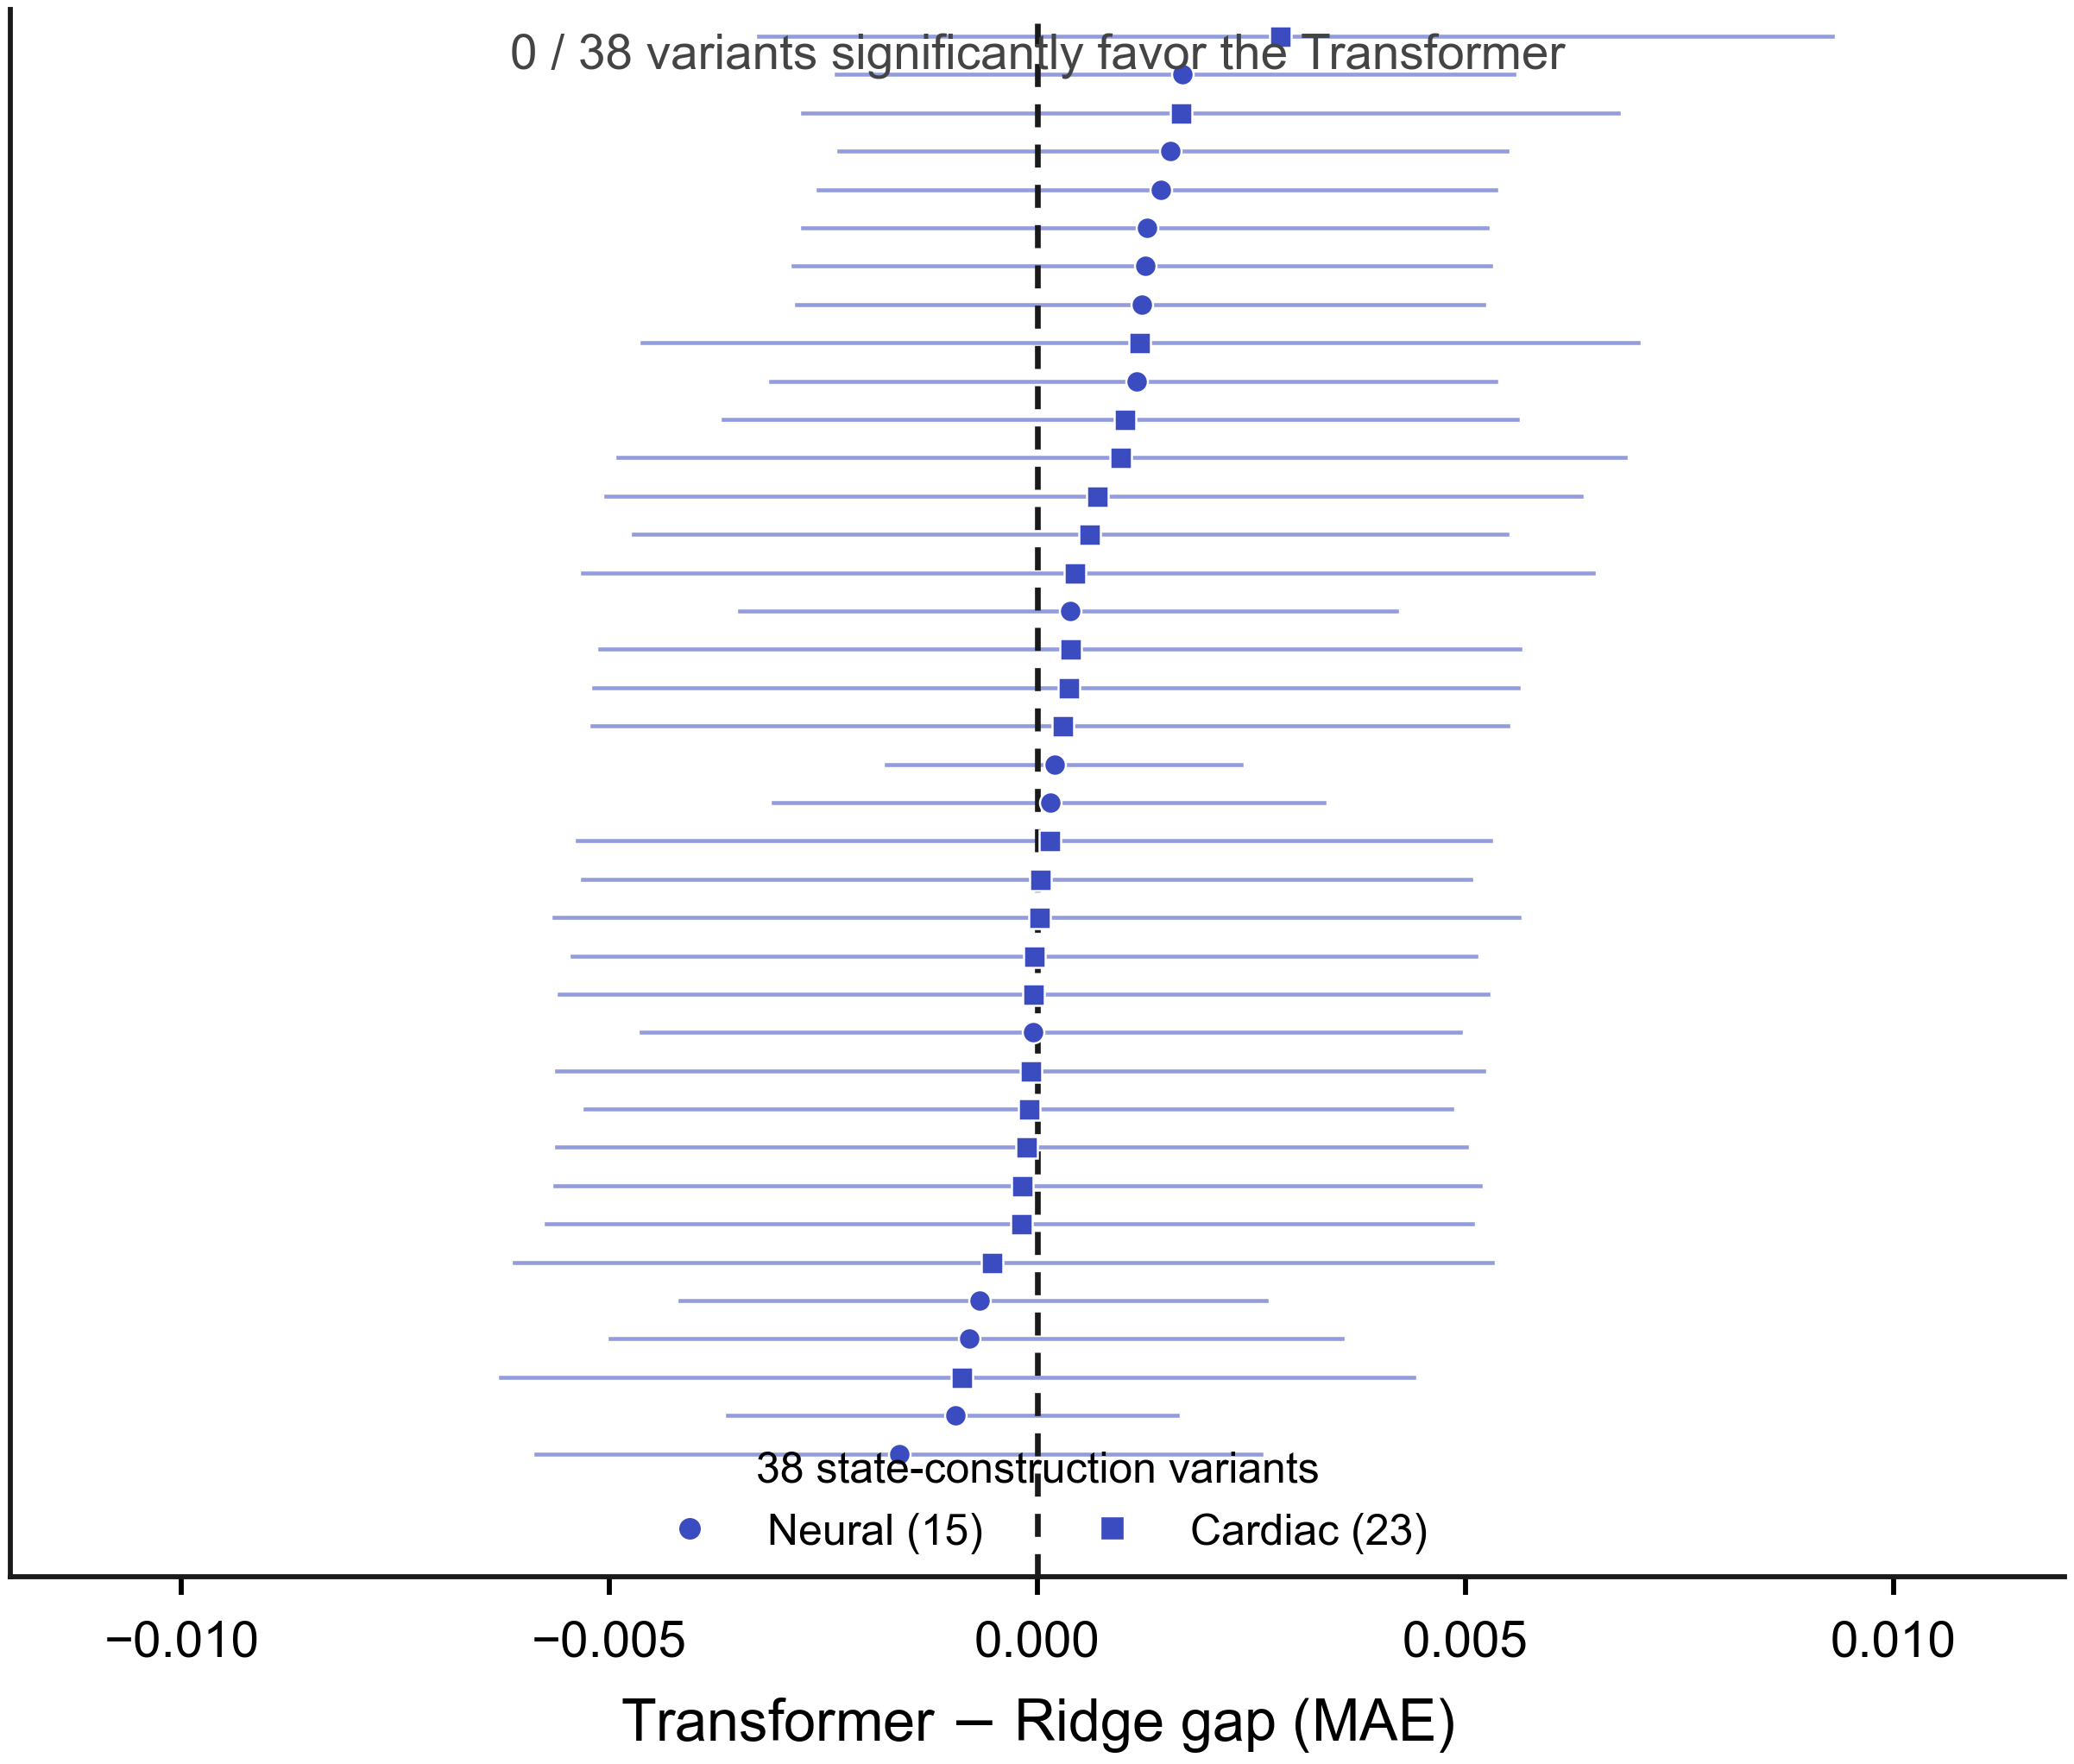
\includegraphics[width=\columnwidth]{figures/fig6_sensitivity.png}
\caption{\textbf{The equivalence is invariant to the state representation.} Paired Transformer$-$Ridge MAE gap (point estimate with $95\%$ CI, $n=20$ seeds) for each of $38$ state-construction variants---per-gene leave-one-out, median and $z$-score aggregation, and an enlarged neural panel---sorted by gap; circles, neural ($15$ variants); squares, cardiac ($23$). Every interval lies within the equivalence margin $|\Delta|<0.01$ and no variant significantly favours the Transformer ($0/38$).}
\label{fig:sensitivity}
\end{figure}

\subsection{Positive Controls: Recovering the Null and Detecting Dependence}
\label{subsec:res_positive}

\subsubsection{Simulation with a known coupling} On simulated differentiation (Eq.~\eqref{eq:sde}), the protocol separates the three constructions sharply (Fig.~\ref{fig:positive}A). Trained on true trajectories, every model reduces held-out error to roughly a fifth of the constant's (Ridge $0.053$, random forest $0.045$, Transformer $0.048$ versus $0.236$ at $N=200$; Holm-corrected $p<10^{-5}$). Trained on independently paired snapshot cells, no model improves significantly on the constant (all Holm-corrected $p>0.2$), as Proposition~\ref{prop:null} requires. Trained on OT-coupled cells, the models recover nearly all of the oracle's accuracy on held-out \emph{true} trajectories (Ridge $0.055$, random forest $0.048$, Transformer $0.051$). At $N=2{,}000$ the picture is unchanged: $0.040$--$0.048$ (true) and $0.044$--$0.049$ (OT-coupled) against $0.226$ for the constant (all $p<0.01$), while independent pairing again yields no improvement (all $p\ge0.48$). Two observations bear on the main analysis. First, even with strong genuine dependence the Transformer is not better than the random forest; on true trajectories it is significantly worse whether trained on true or OT-coupled data (paired Wilcoxon $p<0.01$). Second, the stage-order shuffle leaves the Transformer's error essentially unchanged even here (true coupling, $N=200$: $\overline{\Delta}=-0.0019$, $95\%$ CI $[-0.0042,\,0.0003]$; $N=2{,}000$: $+0.0003$), because the model identifies stage order from the values themselves.

\subsubsection{OT-coupled pseudo-trajectories from the real data} Rebuilding the real-data pseudo-trajectories with OT couplings changes the outcome on both lineages (Fig.~\ref{fig:positive}B). Against the loss-matched reference, the training-mean constant, no model differs significantly under independent pairing on either lineage or sample size; Ridge and the random forest are equivalent to it throughout (all CIs within $\pm0.0032$), as is the Transformer except on the cardiac lineage at $N=200$, where its wider interval ($[-0.0023,\,0.0130]$) extends beyond the margin. Under OT coupling every model beats it: at $N=200$ by $0.012$--$0.018$ MAE on the neural lineage ($p<10^{-4}$) and by $0.012$--$0.013$ for Ridge and the random forest on the cardiac lineage ($p<0.001$; the Transformer's $0.006$ gain is not significant), and at $N=2{,}000$ by $0.014$--$0.018$ on both lineages (all $p<0.01$, the smallest attainable with $10$ seeds). At $N=2{,}000$ on the neural lineage every model beats even the constant median, by $0.010$--$0.012$ ($8$--$9\%$; $p<0.01$). The Transformer again never significantly outperforms the random forest (all paired $p>0.05$).

Together, the three constructions support distinct conclusions. Under \emph{independent pairing}, the protocol recovers the analytical null, in simulation and on both lineages. In \emph{simulation}, it detects temporal dependence that is genuinely present, and OT-coupled training recovers most of it. On \emph{real data with OT coupling}, it detects the dependence that the chosen coupling induces, which is inferred rather than observed. The protocol is therefore not biased toward reporting nulls, and the null of the main analysis is a property of independent pairing, not of the protocol, the two-dimensional state, or the sample size.

\begin{figure*}[!t]
\centering
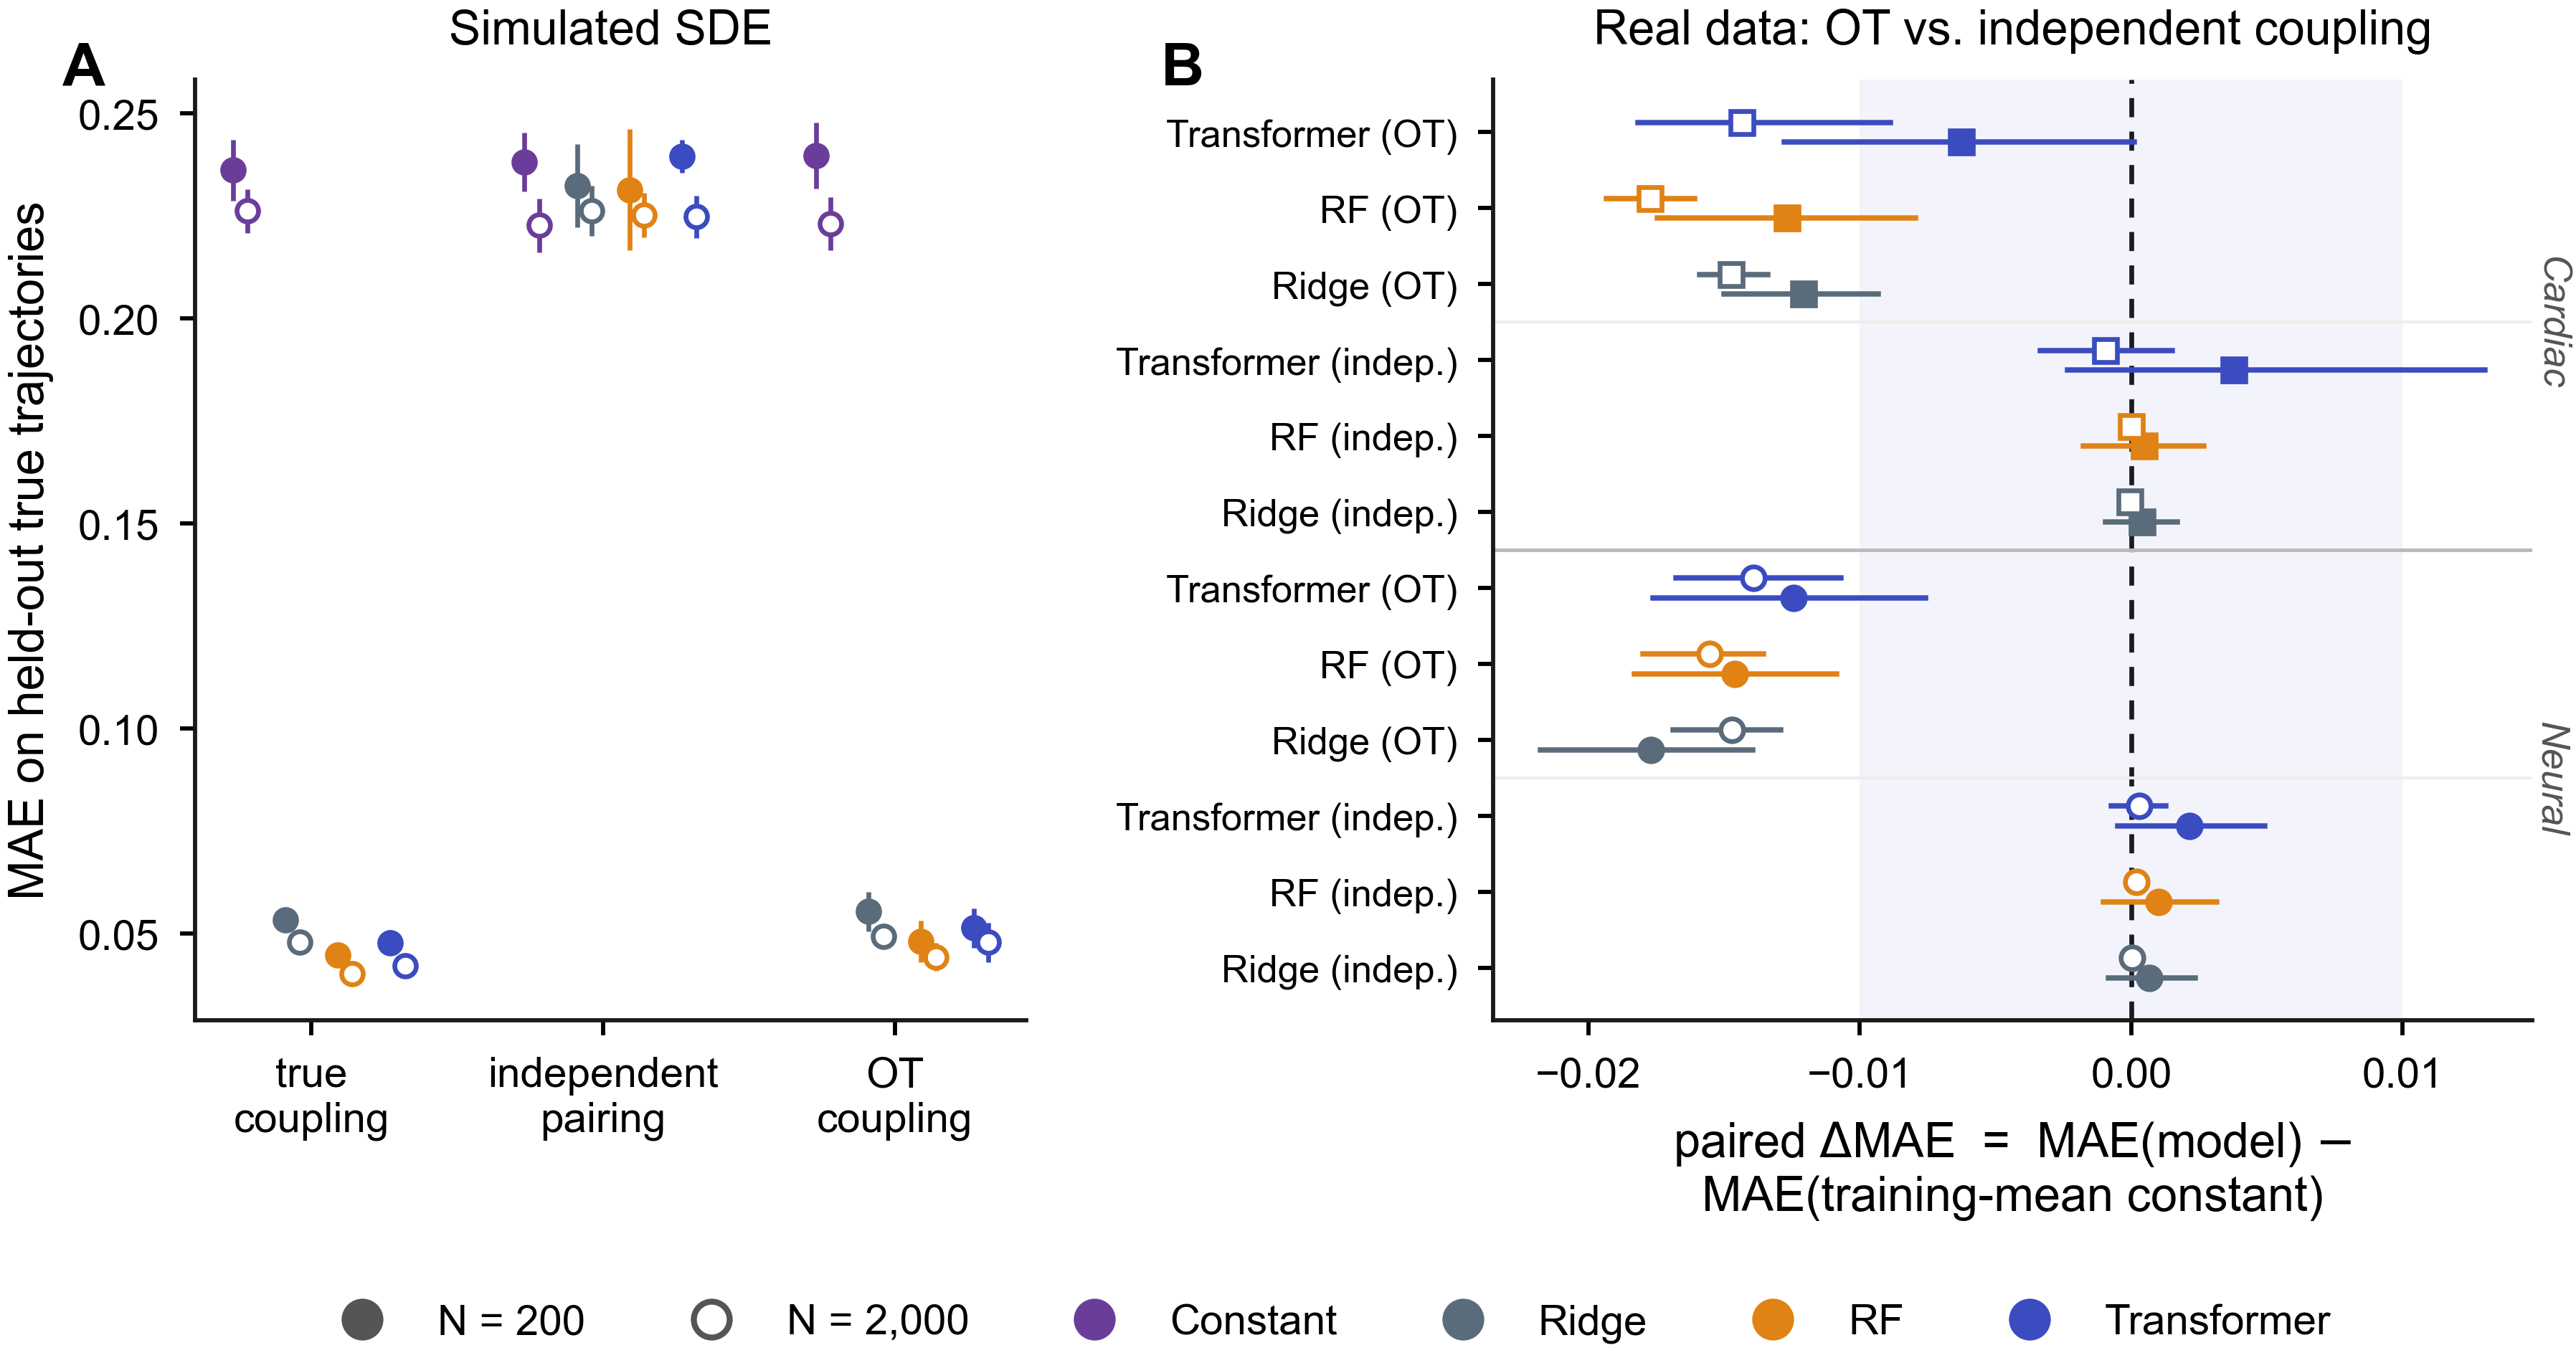
\includegraphics[width=0.92\textwidth]{figures/fig7_positive.png}
\caption{\textbf{Recovering the null and detecting dependence.} \textbf{(A)} Simulated differentiation from a gradient SDE: test MAE (mean\,$\pm$\,s.d.\ over seeds) on held-out \emph{true} trajectories for models trained on true trajectories, independently paired snapshot cells, or OT-coupled snapshot cells; filled markers $N=200$ ($20$ seeds), open markers $N=2{,}000$ ($10$ seeds). \textbf{(B)} Real data: paired difference between each model and the training-mean constant (the input-free optimum of the squared-error training loss), with $95\%$ bootstrap CIs, under independent and OT coupling; circles neural, squares cardiac; filled $N=200$, open $N=2{,}000$. Shaded band, equivalence margin $|\Delta|<0.01$. Negative values indicate that the model extracts information from its inputs, which occurs only under OT coupling; on real data this reflects dependence induced by the coupling, which is not shown to be biological.}
\label{fig:positive}
\end{figure*}

\subsection{Case Study: A Leaky Evaluation Reports the Opposite}
\label{subsec:res_leakage}

Re-running the evaluation pipeline of our earlier study~\cite{kanu2026transformer} for its single seed yields a test MAE of $0.081$ for the Transformer against $0.100$ for the best classical baseline, an apparent $+19.4\%$ advantage. The gap arises from inconsistent index handling that let $22$ of the Transformer's $30$ nominal test trajectories appear in its training set, while the baselines were scored leakage-free (Sec.~S7, Fig.~S2). Re-scoring every model on the identical trajectories under one consistent split turns the advantage into a $2.0\%$ Transformer deficit relative to the best classical baseline (Table~\ref{tab:leakage}). On independently paired data, where Proposition~\ref{prop:null} rules out any systematic advantage, a gain of this size must come from sampling variation or the evaluation procedure; one shared split, programmatic generation of every number, and a constant baseline that no model should beat each help expose such discrepancies.

\begin{table}[!t]
\centering
\caption{Single-seed MAE on the neural lineage under the leaky evaluation and after re-scoring all models on the identical frozen trajectories with a consistent split. The apparent advantage inverts once the leakage is removed.}
\label{tab:leakage}
\footnotesize
\setlength{\tabcolsep}{6pt}
\begin{tabular}{lcc}
\toprule
\textbf{Model} & \textbf{Leaky eval.} & \textbf{Leakage-free} \\
\midrule
Ridge & 0.100 & 0.0843 \\
Random Forest & 0.102 & 0.0954 \\
Transformer & 0.081 & 0.0861 \\
Mechanistic ODE & 0.433 & 0.4147 \\
\midrule
\textbf{Transformer vs.\ best baseline} & \textbf{+19.4\%} & \textbf{$-2.0\%$} \\
\bottomrule
\end{tabular}
\end{table}

\section{Discussion}
\label{sec:discussion}

What a single-cell forecasting benchmark can detect depends more on how cells are linked across time than on which model is used. Independent pairing makes the late state independent of the earlier states, so the optimal forecast is a constant (Proposition~\ref{prop:null}). This is not how cross-sectional time courses are usually linked---optimal-transport methods infer a coupling~\cite{schiebinger2019optimal}---but it is the simplest construction available when no lineage is measured, and it was used in the original study~\cite{kanu2026transformer}. The data confirm every prediction of the proposition: the constant median outperforms every trained model, the trained models perform no better than the training mean their loss favours, destroying stage order changes nothing, and added flexibility, in the ODE or an under-regularized forest, fits noise. Proposition~\ref{prop:null} makes this outcome predictable before any experiment; the empirical analyses are valuable not as a discovery of the null but as a check that the protocol reports it correctly, and as a demonstration of how a leaky evaluation reports the opposite.

\subsection{Coupling, Not Capacity, Sets What Can Be Detected}
The positive controls separate two questions that the original design conflated: whether the benchmark contains temporal information, and whether a given model can use it. The first is determined by the coupling: the same cells, state, and models move from a null to a significant advantage over the input-free baseline when independent pairing is replaced by OT coupling, on both lineages and at both sample sizes, although these data cannot establish whether the induced dependence is biologically valid. On the second, the Transformer was never significantly better than the random forest and was significantly worse in simulation, even with genuine dependence and ten times more trajectories. This is not an indictment of Transformers: the model trains stably and matches Ridge, but this short, low-dimensional task provides no evidence of a structural advantage for it. The difficulty lies in evaluating any model on a task whose construction precludes the signal it targets, compounded by leakage and single-seed reporting that together can manufacture an apparent gain.

\subsection{Implications for Single-Cell Forecasting Practice}
Four inexpensive practices would have exposed the problem. First, a single, consistent split shared identically across models; the asymmetry here affected only one model. Second, multi-seed reporting with paired effect sizes and equivalence reasoning; the spurious ranking was smaller than the seed-to-seed noise. Third, controls should be validated before they are trusted: the stage-order shuffle proved insensitive in the positive control because stage identity can be read from the state values, so it is informative only when stages cannot be distinguished by value. Fourth, an input-independent baseline matched to the evaluation metric---here the training median---should be reported alongside any learned model, and a model should be shown to outperform it, not merely a linear regressor, before forecasting ability is claimed.

\subsection{Limitations and Scope}
First, the forecasting target is a two-dimensional marker-program state, a strong compression of the transcriptome. The null does not depend on it---Proposition~\ref{prop:null} holds for any representation of independently paired cells, and the $38$-variant sweep and the transcriptome-wide OT couplings agree---but the positive-control results describe forecasting of this compressed state only. Second, the dependence induced by OT coupling on real data is inferred rather than observed; settings with measured lineage, such as barcoded time courses~\cite{weinreb2020lineage}, are needed to test biological forecasting ability. Third, the stages are days to weeks apart, far longer than the hours resolved by RNA velocity or metabolic labelling (Table~\ref{tab:rigor}), so any temporal information must come from the coupling rather than within-cell kinetics. Fourth, models are trained with squared error but scored by absolute error, and point rather than distributional predictions are evaluated; the mean- and median-constant references make the first explicit. Finally, the $N=2{,}000$ analyses use $10$ rather than $20$ seeds, which limits the smallest attainable $p$-value but not the direction or size of the effects.

\section{Conclusion}
\label{sec:conclusion}
Whether a single-cell forecasting benchmark can reveal any model's skill is decided by how cells are coupled across time. Under independent pairing the optimal forecast is a constant; across two lineages, a Transformer, a random forest, and a linear model were statistically equivalent and all were outperformed by the training median, and an apparent Transformer advantage traced to train--test leakage. With a known coupling the identical protocol detects recoverable dependence, and with optimal-transport coupling of real cells it detects the dependence that coupling induces---in neither case finding an advantage for the Transformer over a random forest. Forecasting benchmarks built on cross-sectional snapshots should therefore state their coupling, compare every model with a metric-matched input-independent baseline, evaluate leakage-safely over many seeds with explicit equivalence tests, and validate their controls where temporal dependence is known to exist. Only an evaluation that can fail to find an effect, and has been shown able to find one, can credibly report either.

\section*{Availability of Data and Materials}

The dopaminergic-neuron scRNA-seq data~\cite{jerber2021population} are available from the European Nucleotide Archive (ERP121676; BioProject PRJEB38269), with genotype-linked data under managed access in the European Genome--phenome Archive (EGAS00001002885) and processed count files on Zenodo (record 4333872). The cardiomyocyte data~\cite{elorbany2022single} are available from the Gene Expression Omnibus (GSE175634). No new sequencing data were generated. All code, per-seed result files, the per-cell embeddings used for the OT couplings, and scripts that regenerate every figure and table are available under the MIT license at \url{https://github.com/xaviwho/leakage-safe-benchmark}.

\ifCLASSOPTIONcompsoc
  \section*{Acknowledgments}
\else
  \section*{Acknowledgment}
\fi

This work was partly supported by Innovative Human Resource Development for Local Intellectualization program through the IITP grant funded by the Korea government (MSIT) (IITP-2026-RS-2020-II201612, 25\%) and by Priority Research Centers Program through the NRF funded by the MEST (2018R1A6A1A03024003, 25\%) and by the MSIT, Korea, under the ITRC support program (IITP-2026-RS-2024-00438430, 25\%) and by Basic Science Research Program through the National Research Foundation of Korea(NRF) funded by the Ministry of Education(RS-2025-25431637, 25\%).

\bibliographystyle{IEEEtran}
\bibliography{sn-bibliography}

% Author biographies are required in the final IEEE version. Uncomment and
% complete; use IEEEbiography with a photo file for the final submission.
%
% \begin{IEEEbiographynophoto}{Victor Ikenna Kanu}
% Biography text here.
% \end{IEEEbiographynophoto}
%
% \begin{IEEEbiographynophoto}{Ihunanya Udodiri Ajakwe}
% Biography text here.
% \end{IEEEbiographynophoto}
%
% \begin{IEEEbiographynophoto}{Josiah Ayoola Isong}
% Biography text here.
% \end{IEEEbiographynophoto}
%
% \begin{IEEEbiographynophoto}{Simeon Okechukwu Ajakwe}
% Biography text here.
% \end{IEEEbiographynophoto}
%
% \begin{IEEEbiographynophoto}{Dong-Seong Kim}
% Biography text here.
% \end{IEEEbiographynophoto}

\end{document}
